\documentclass[10pt]{article}
\usepackage[a4paper,margin=20mm]{geometry}
\usepackage[T1]{fontenc}
\usepackage[utf8]{inputenc}
\usepackage{lmodern}
\usepackage{microtype}
\usepackage{amsmath,amssymb}
\usepackage{booktabs,longtable,array}
\usepackage{graphicx,float,caption}
\usepackage{enumitem}
\usepackage{xcolor}
\usepackage[unicode]{hyperref}
\usepackage{fancyhdr}

\graphicspath{{figures/}}
\setlist{nosep,leftmargin=*}
\hypersetup{
  colorlinks=true,
  linkcolor=black,
  urlcolor=blue,
  pdftitle={Numerical Normality Audit of the Exponentially Weighted Endpoint Coordinate},
  pdfauthor={Paweł Małmyga},
  pdfsubject={Finite-lookback simulation study of Gaussian approximation for the exponentially weighted endpoint coordinate},
  pdfkeywords={endpoint coordinate, normal approximation, finite lookback, Q-Q plot, Monte Carlo, RSI}
}
\pagestyle{fancy}
\fancyhf{}
\lhead{Numerical normality audit}
\rhead{Computational supplement}
\cfoot{\thepage}
\setlength{\headheight}{14pt}

\newcommand{\E}{\mathbb{E}}
\newcommand{\Var}{\operatorname{Var}}
\newcommand{\Prob}{\mathbb{P}}

\title{\textbf{Numerical Normality Audit of the\
Exponentially Weighted Endpoint Coordinate}\\[5pt]
\large Finite-lookback scale calibration, Q-Q geometry, and tail behavior}
\author{Pawe{\l} Ma{\l}myga\\
\small Reproducible computational supplement}
\date{September 2026}

\begin{document}
\maketitle

\begin{abstract}
This report asks a finite-sample question not settled by asymptotic normality
alone.  For the stationary log-odds endpoint coordinate
\(L_t=\log(U_t/D_t)\), does standardization by the asymptotic scale or by the
derived law-specific finite-lookback correction produce an approximately
standard normal marginal distribution at practically relevant lookbacks?

The audit evaluates 216 million coordinate values: 3 million retained time
points for each of 72 law-lookback combinations.  The laws are Gaussian,
Laplace, and standardized Student \(t_\nu\) with \(\nu=4,5,6,8\); the lookbacks
are \(2,3,5,8,13,21,35,55,89,144,233,377\).  The analysis reports variance,
skewness, excess kurtosis, Kolmogorov distance, truncated quantile-grid mean
absolute error, normal Q-Q regressions, central coverage, and tail frequencies.  An empirical
variance ``oracle'' is included only to distinguish scale error from residual
shape error.

The result is not exact finite-\(n\) Gaussianity.  The law-specific correction
usually removes most of the scale error, and the remaining shape approaches a
Gaussian form with increasing lookback.  Gaussian and Laplace cases are
already close in Kolmogorov distance at short horizons, although their
positive excess kurtosis remains visible.  Student \(t_4\) is the important
short-horizon exception: its first shift vanishes (\(K_4=0\)), so the
first-order corrected scale coincides with the asymptotic scale and substantially over-scales
\(n=2\) and \(n=3\).  Across all laws the Q-Q grids
become visually close to linear at moderate lookbacks, but variance
normalization should not be described as an exact Gaussianizing transform.
\end{abstract}

\section{Question and answer}

The analytical manuscript proves an asymptotic Gaussian limit and a
law-dependent finite-lookback variance expansion under its stated
assumptions.  Neither statement says that the transformed statistic is exactly
normal at any fixed lookback.  This audit therefore separates three questions:

\begin{enumerate}
\item Does the proposed scale make the variance close to one?
\item After removing scale error, is the remaining distributional shape close
      to standard normal?
\item Is the resulting distribution stable enough across lookbacks to support
      percentile comparisons?
\end{enumerate}

The numerical answer is:

\begin{itemize}
\item \textbf{Scale:} the law-specific correction is much better than the
      first-order asymptotic scale at short and moderate lookbacks for Gaussian
      and Laplace innovations.  The Student first-shift correction can be good,
      poor, or directionally wrong at \(n=2\), depending on \(\nu\).
\item \textbf{Shape:} finite-\(n\) distributions retain excess kurtosis.  The
      deviation is modest for Gaussian and Laplace inputs and decreases with
      \(n\).  The oracle diagnostic confirms that standardizing the variance
      does not eliminate all non-Gaussian shape.
\item \textbf{Use:} the coordinate is an increasingly accurate Gaussian pivot,
      not an exact small-sample pivot.  For practical small-\(n\) thresholds,
      law-specific empirical percentiles remain safer than universal normal
      cutoffs.
\end{itemize}

\section{Statistic and scales}

For gain \(\alpha=1/n\), let
\begin{align}
U_t&=(1-\alpha)U_{t-1}+\alpha\max(\varepsilon_t,0),\\
D_t&=(1-\alpha)D_{t-1}+\alpha\max(-\varepsilon_t,0),
\end{align}
and define
\begin{equation}
L_t^{(n)}=\log\frac{U_t}{D_t}.
\end{equation}
For a centered innovation law with standard deviation \(\sigma\) and
\(m_1=\E|\varepsilon|\), the asymptotic scale is
\begin{equation}
C_F=\frac{\sqrt{2}\,\sigma}{m_1}.
\end{equation}

Three normalizations are compared:
\begin{align}
Z_{n}^{\mathrm{asym}}&=\frac{\sqrt n}{C_F}L_t^{(n)},\\
Z_{n}^{\mathrm{corr}}&=\frac{\sqrt{g_F(n)}}{C_F}L_t^{(n)},\\
Z_{n}^{\mathrm{oracle}}&=
\frac{L_t^{(n)}-\overline L_n}{s(L_n)}.
\end{align}
The oracle is not a proposed normalization.  It uses the same simulation sample
to center and scale the statistic and therefore answers only whether the shape,
after scale removal, resembles a normal distribution.

For Gaussian and Laplace laws, the correction uses
\begin{equation}
g_F(n)=n-K_F+\frac{A_F}{n}+\frac{B_F}{n^2}.
\end{equation}
For Student laws it uses only the first-shift correction developed in the
companion conventional technical note,
\(g_\nu(n)=n-K_\nu\).  This correction remains outside Lean, and that
distinction is material at small \(n\).

\begin{table}[H]
\centering
\caption{Scale constants and correction formulas used by the audit.}
\label{tab:constants}
\begin{tabular}{lrrl}
\toprule
Law & $C_F$ & $K_F$ & Correction used \\
\midrule
Gaussian & 1.772454 & 1.593657 & $n-K_F+A_F/n+B_F/n^2$ \\
Laplace & 2.000000 & 1.333333 & $n-K_F+A_F/n+B_F/n^2$ \\
Student-t4 & 2.000000 & -0.000000 & $n-K_F$ (analytic note) \\
Student-t5 & 1.923825 & 0.959710 & $n-K_F$ (analytic note) \\
Student-t6 & 1.885618 & 1.222222 & $n-K_F$ (analytic note) \\
Student-t8 & 1.847521 & 1.400000 & $n-K_F$ (analytic note) \\
\bottomrule
\end{tabular}
\end{table}


\section{Simulation design}

\subsection{Path construction}

For each innovation law, one reproducible path is generated with seed
\texttt{20260923}.  The same innovation path is used across lookbacks within a
law, making comparisons paired.  The Wilder recursions start from zero and the
first \(32\max(n)=12064\) observations are discarded.  At \(n=377\), the
remaining weight of the zero initialization is below approximately
\(\exp(-32)\); it is smaller for every other lookback.

After burn-in, 3,000,000 time points are retained for every law-lookback pair.
These observations represent the stationary marginal distribution but are not
independent.  Standard i.i.d. normality-test p-values would therefore be
miscalibrated and, at this sample size, scientifically unhelpful.  They are not
reported.

\subsection{Metrics}

The audit reports:
\begin{itemize}
\item mean, variance, skewness, and excess kurtosis;
\item one-sample Kolmogorov distance from \(N(0,1)\);
\item mean absolute error on a dense normal-quantile grid over probabilities
      0.005 through 0.995.  This is a truncated quantile-grid diagnostic,
      stored as \texttt{wasserstein\_grid}, not the full \(W_1\) distance on
      the real line;
\item a linear Q-Q fit over probabilities 0.005 through 0.995: intercept,
      slope, and \(R^2\);
\item coverage of the nominal 95\% and 99\% normal intervals;
\item \(\Prob(|Z|>2)\) and \(\Prob(|Z|>3)\);
\item central-quantile RMSE relative to the \(n=377\) distribution.
\end{itemize}

The path is partitioned into 192 contiguous blocks.  Block-to-block variation
provides correlation-aware Monte Carlo standard errors for moments, coverage,
and tail frequencies.  The longest-lookback block contains more than 41
lookbacks.  These errors measure simulation stability; they are not a claim
that the blocks are exactly independent.

Complete aggregate outputs, quantile grids, block summaries, and
representative draws are provided in the accompanying reproducibility
package; see Appendix~\ref{app:reproducibility}.

\section{Validation of the computation}

The computational validation verifies all of the following:
\begin{itemize}
\item all 216 law-lookback-normalizer rows are present with unique keys;
\item every required numerical field is finite;
\item the reported variances satisfy the scale identity to a maximum absolute
      error of \(1.34\times10^{-15}\);
\item no comparison between the first and second halves of the block sequence
      exceeds three pooled block standard errors.  The maximum absolute split
      diagnostic is 2.82.
\end{itemize}
These checks assess completeness, algebraic consistency, and simulation
stability; they are not a formal proof of the model or unadjusted multiple
hypothesis tests.  The machine-readable checks and file inventory are
documented in Appendix~\ref{app:reproducibility} and in the repository.

\section{Results}

\subsection{Variance calibration}

Figure~\ref{fig:variance-calibration} compares the asymptotic and finite-\(n\)
scales.  For Gaussian and Laplace inputs the corrected variance is materially
closer to one over most of the grid.  At \(n=2\), the Gaussian fourth-order
approximation still leaves variance 1.0847, while the Laplace value is 1.0084.
For Laplace innovations, a small residual over-dispersion of approximately
1--2\% remains across much of the moderate-lookback grid.  This is a useful
warning: a fourth-order large-\(n\) expansion can be accurate at a very small
horizon without being an exact finite-\(n\) calibration.

For Student inputs, the first shift is visibly asymptotic.  At \(n=2\), the
corrected variances are 2.2672, 1.2589, 0.9670, and 0.7719 for
\(\nu=4,5,6,8\), respectively.  The fact that \(t_6\) happens to be close to one
does not make the formula uniformly small-sample accurate across \(\nu\).
For \(\nu=4\), \(K_4=0\) and hence \(g_4(n)=n\): the corrected and asymptotic
normalizations are identical throughout the grid.  Its small-\(n\)
over-dispersion therefore records a limitation of the first-shift
approximation, not the effect of a distinct finite-\(n\) rescaling.

\begin{figure}[H]
\centering
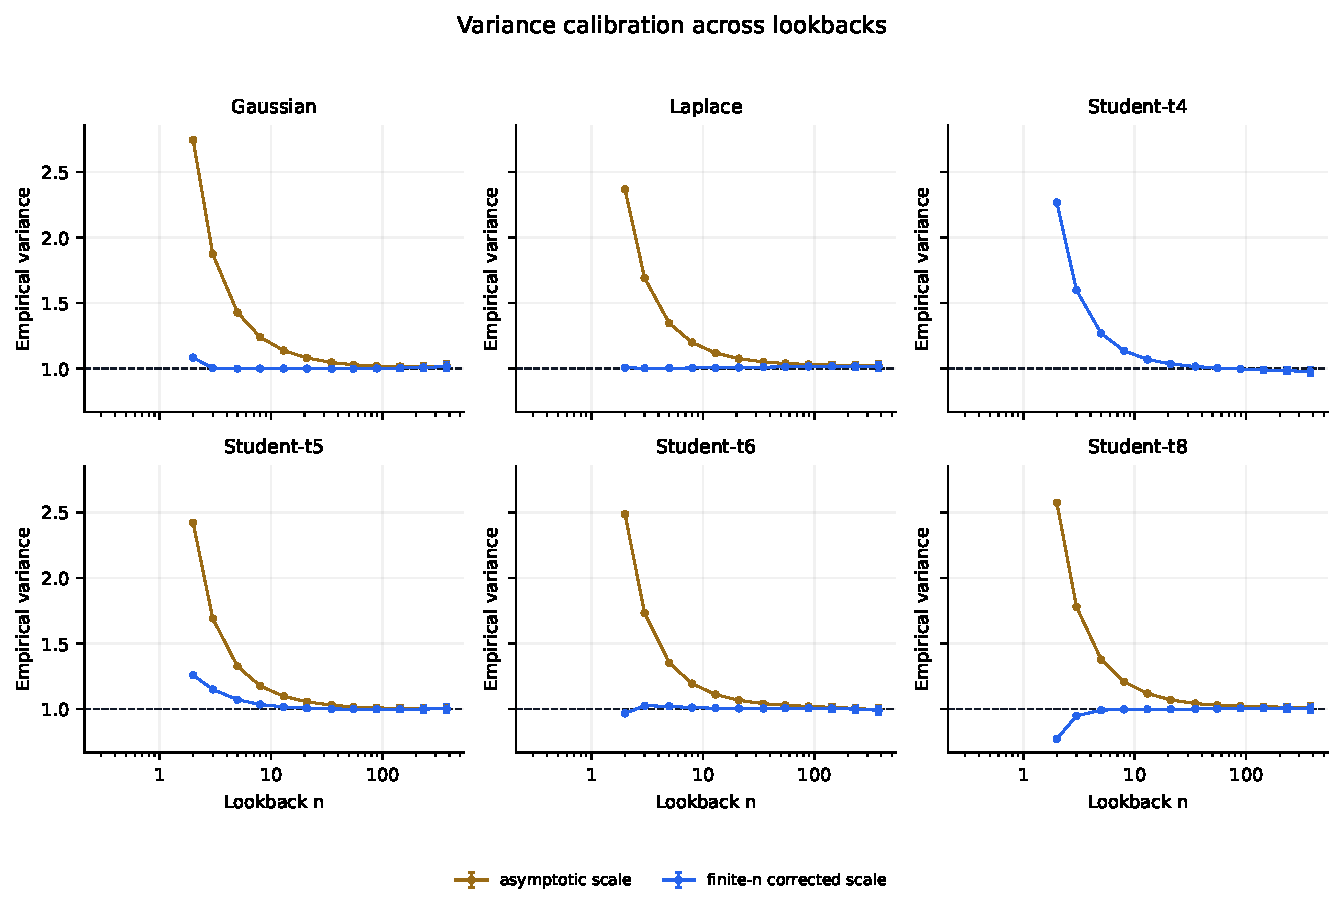
\includegraphics[width=0.98\textwidth]{variance_calibration.pdf}
\caption{Empirical variance under the first-order asymptotic scale and the
law-specific finite-lookback scale. Error bars are 95\% block Monte Carlo
intervals. The oracle is omitted because its sample variance equals one by
construction.}
\label{fig:variance-calibration}
\end{figure}

\subsection{Scale error versus shape error}

At \(n=2\), the asymptotic scale produces Kolmogorov distances near 0.09--0.11
for every law.  The finite-\(n\) correction reduces that distance to 0.0056 for
Gaussian and 0.0077 for Laplace.  Student results depend strongly on \(\nu\):
0.0879 for \(t_4\), 0.0184 for \(t_5\), 0.0143 for \(t_6\), and 0.0417 for
\(t_8\).

After empirical variance normalization, all six \(n=2\) Kolmogorov distances
fall in the narrow interval 0.0087--0.0113.  This is the clearest diagnostic
separation in the study.  Most of the dramatic Student \(t_4\) error is scale
error, not an exceptionally distorted central shape.  Nevertheless, all six
laws have positive excess kurtosis between 0.54 and 0.67 at \(n=2\), so the
oracle distributions are not exactly Gaussian.

\begin{table}[H]
\centering
\caption{At $n=2$, comparison of scale error with residual shape. The oracle column uses sample centering and variance and is diagnostic only.}
\label{tab:n2-diagnostic}
\begin{tabular}{lrrrrr}
\toprule
Law & Var corr. & KS asym. & KS corr. & KS oracle & Kurtosis \\
\midrule
Gaussian & 1.0847 & 0.1087 & 0.0056 & 0.0113 & 0.6665 \\
Laplace & 1.0084 & 0.0945 & 0.0077 & 0.0087 & 0.5355 \\
Student-t4 & 2.2672 & 0.0879 & 0.0879 & 0.0101 & 0.6256 \\
Student-t5 & 1.2589 & 0.0953 & 0.0184 & 0.0104 & 0.6172 \\
Student-t6 & 0.9670 & 0.0986 & 0.0143 & 0.0103 & 0.6098 \\
Student-t8 & 0.7719 & 0.1021 & 0.0417 & 0.0107 & 0.6367 \\
\bottomrule
\end{tabular}
\end{table}


\begin{figure}[H]
\centering
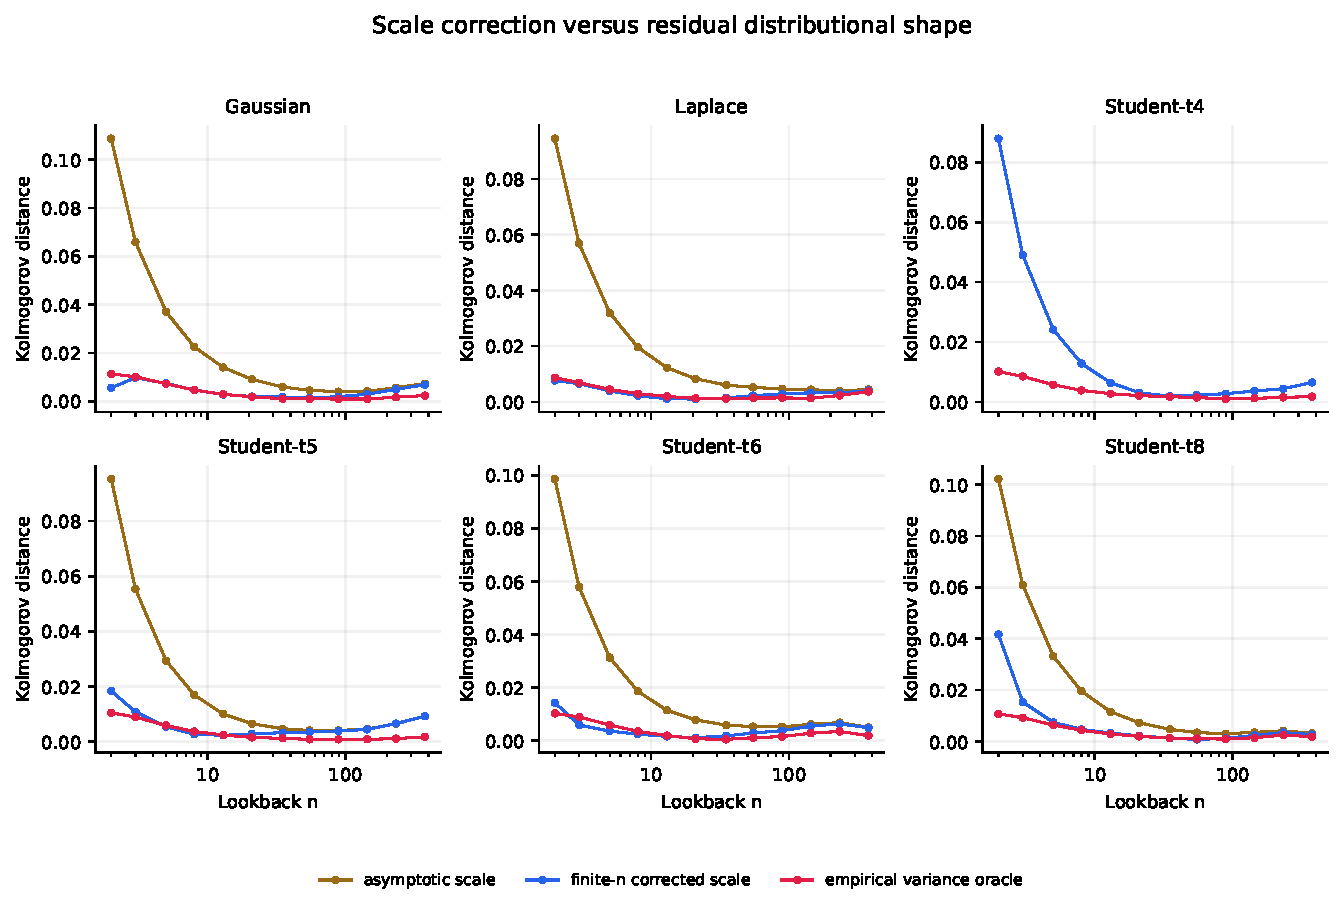
\includegraphics[width=0.98\textwidth]{normalizer_ks_comparison.pdf}
\caption{Kolmogorov distance for the asymptotic, finite-\(n\) corrected, and
oracle scales. The gap between corrected and oracle curves measures scale error;
the oracle curve retains pure finite-\(n\) shape error plus Monte Carlo noise.}
\label{fig:ks-comparison}
\end{figure}

\subsection{Convergence with lookback}

By \(n=13\), the corrected Kolmogorov distances are 0.0028 (Gaussian), 0.0011
(Laplace), 0.0064 (Student \(t_4\)), 0.0023 (Student \(t_5\)), 0.0016 (Student
\(t_6\)), and 0.0033 (Student \(t_8\)).  By \(n=55\), every corrected distance
is below 0.0035.  At the largest lookbacks the descriptive distance can rise
slightly.  This is consistent with the decreasing effective number of nearly
independent states and with Monte Carlo variability in both variance and the
empirical CDF.  The oracle and block diagnostics do not isolate a single cause,
but the observed rise is not evidence of a reversal of the asymptotic result.

The Q-Q regressions are almost perfectly linear in the center even at small
lookbacks.  At \(n=2\), corrected Q-Q slopes range from 0.868 for Student
\(t_8\) to 1.488 for Student \(t_4\), while every reported central-grid
\(R^2\) exceeds 0.998.  Thus a visually straight Q-Q line can coexist with a
materially wrong scale and non-Gaussian tails.  Slope, kurtosis, coverage, and
tail frequency must be read together.

\begin{figure}[H]
\centering
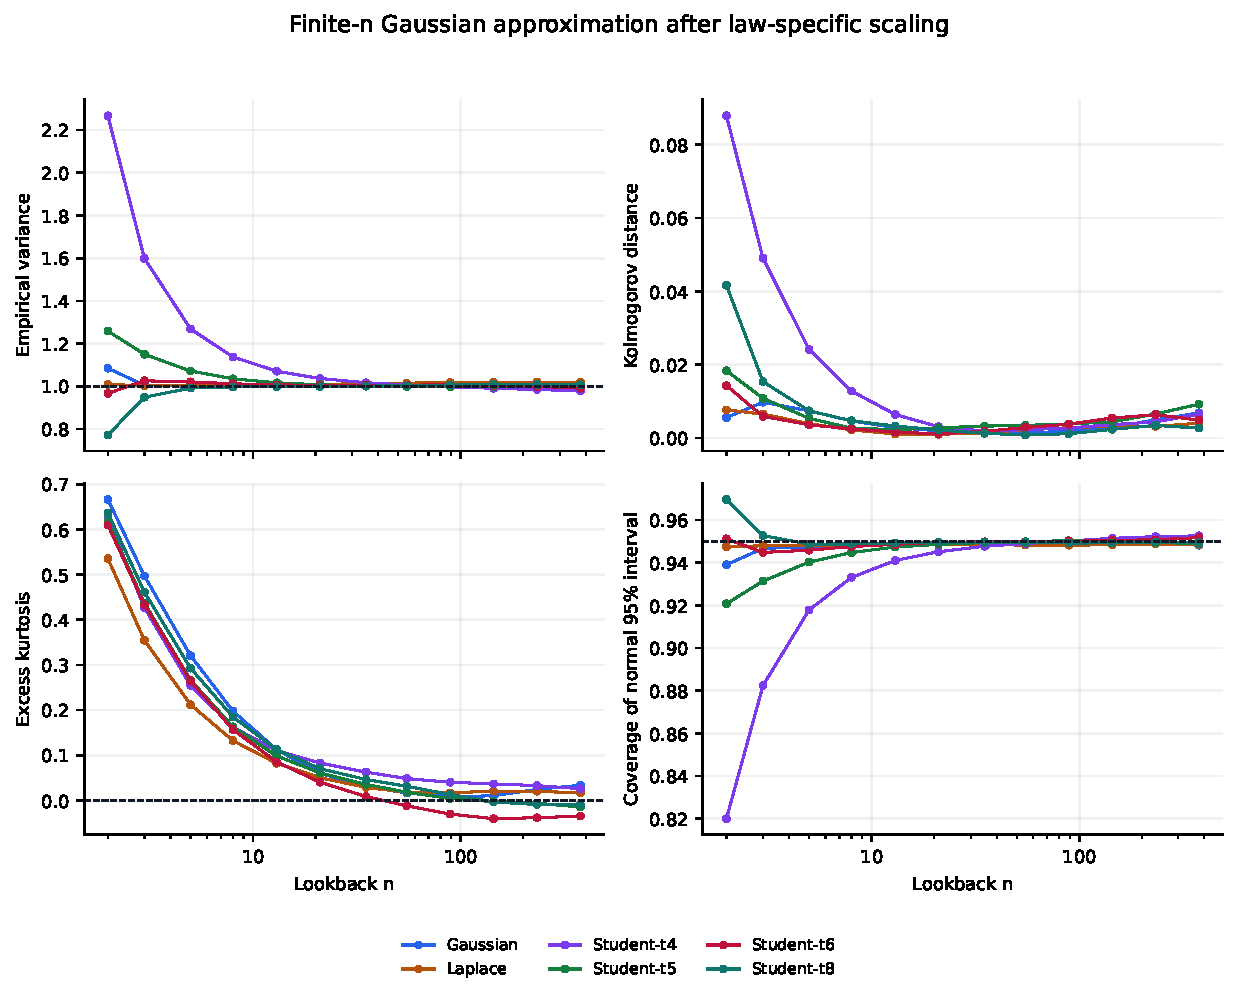
\includegraphics[width=0.98\textwidth]{overview_corrected_metrics.pdf}
\caption{Variance, Kolmogorov distance, excess kurtosis, and nominal 95\%
coverage after the finite-lookback correction. The dashed lines mark standard
normal reference values where applicable.}
\label{fig:overview}
\end{figure}

\subsection{Tail behavior}

The standard normal benchmark is
\(\Prob(|Z|>3)\approx0.00270\).  Gaussian input at \(n=2\) produces 0.00819
after correction, and Laplace input produces 0.00589.  Student \(t_4\) reaches
0.04879 because its small-\(n\) scale is severely over-dispersed.  At moderate
lookbacks the values move toward the normal benchmark, with residual
differences that agree with the excess-kurtosis pattern.

\begin{figure}[H]
\centering
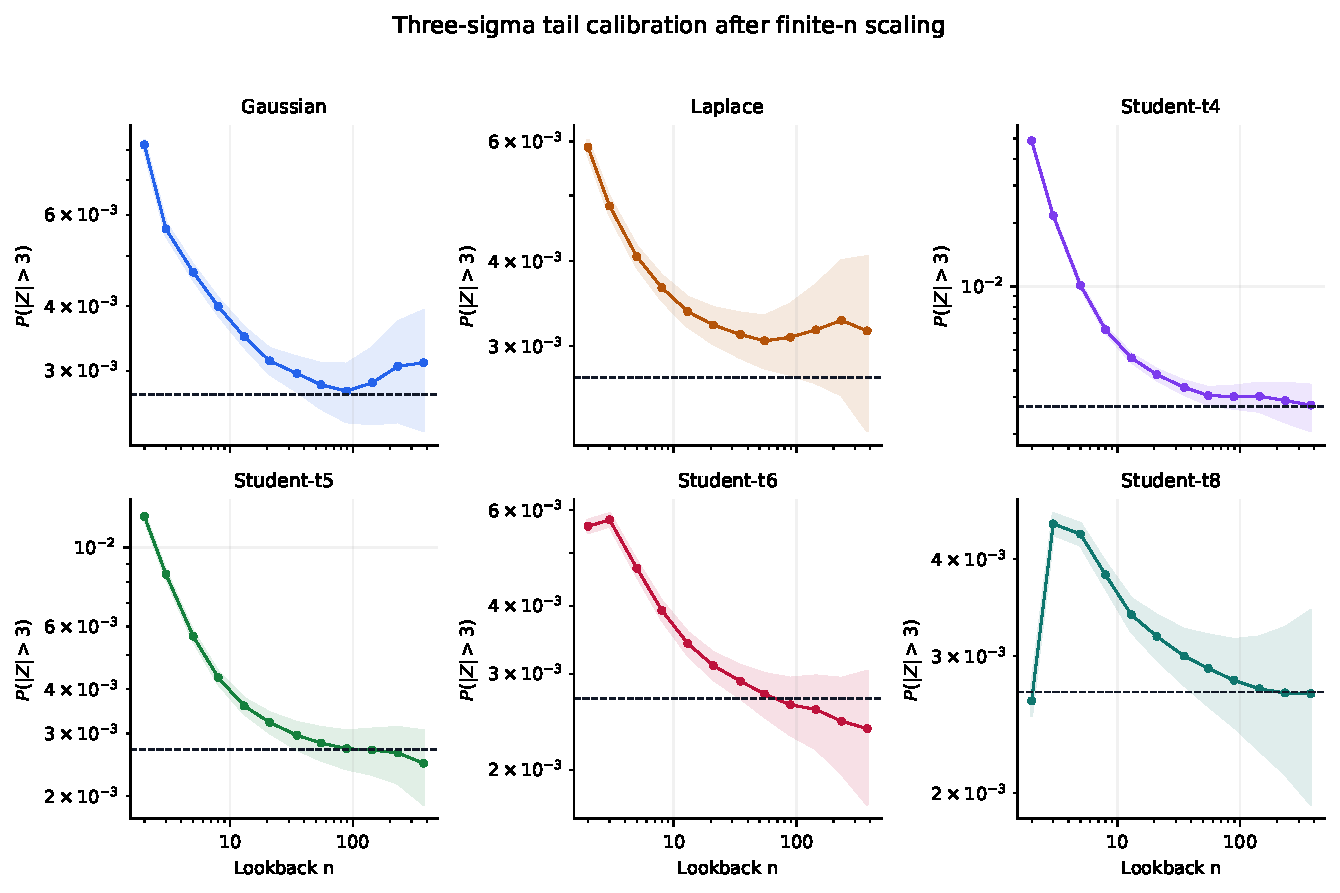
\includegraphics[width=0.98\textwidth]{three_sigma_tail_calibration.pdf}
\caption{Three-sigma tail frequencies on a logarithmic scale. Shading shows
95\% block Monte Carlo intervals; the dashed line is the standard normal tail
probability.}
\label{fig:tail}
\end{figure}

\subsection{Percentile stability}

The percentile heatmaps show empirical minus normal quantiles after the
finite-lookback correction.  Warm and cool bands at \(n=2\) reflect the joint
effect of scale error and finite-\(n\) tail shape.  Errors contract rapidly for
Gaussian and Laplace inputs.  Student \(t_4\) needs a longer horizon because
the first-shift correction leaves substantial variance error at the smallest
lookbacks.

\begin{figure}[H]
\centering
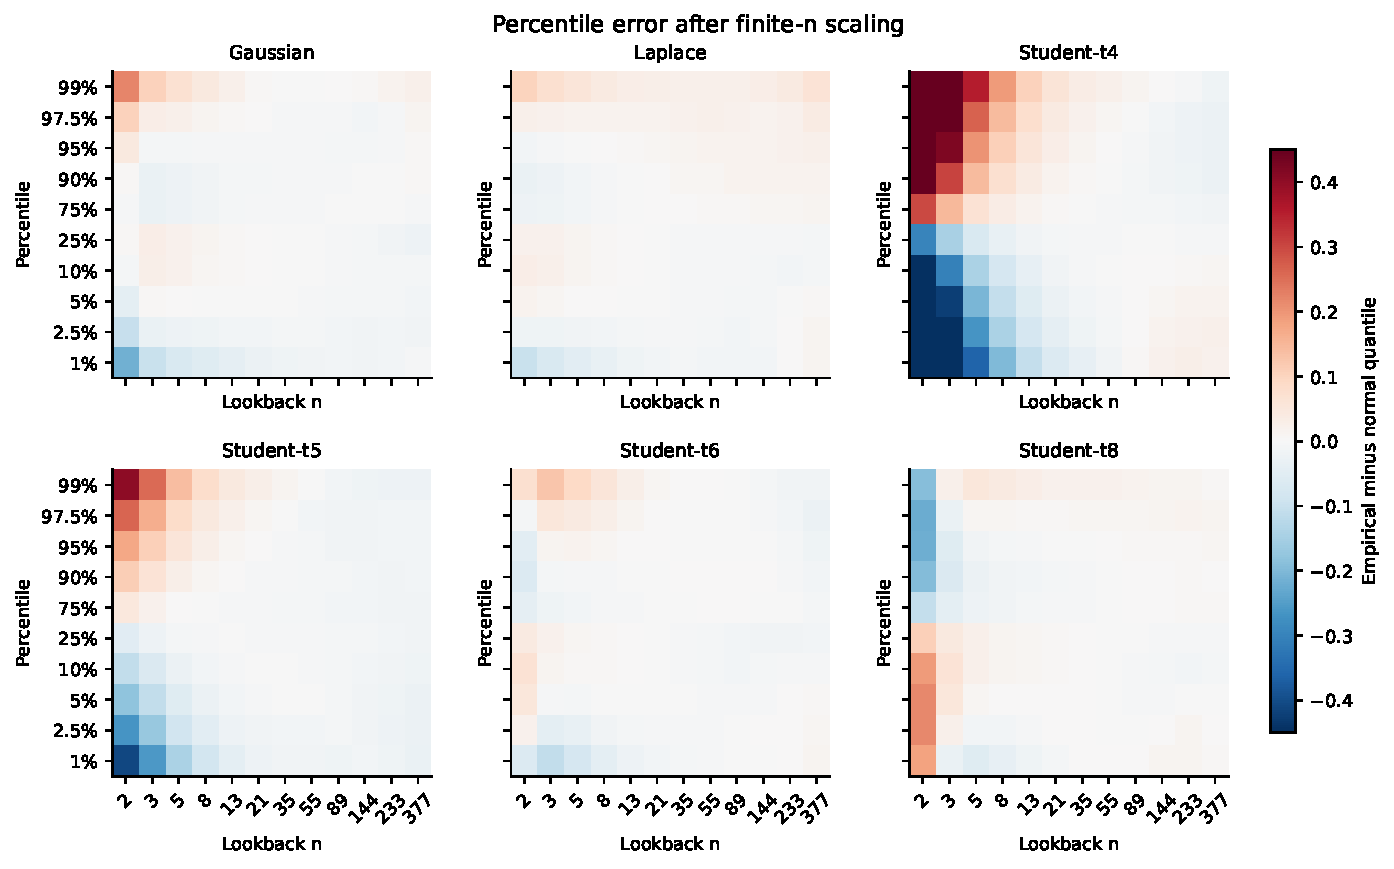
\includegraphics[width=0.98\textwidth]{percentile_error_heatmaps.pdf}
\caption{Difference between empirical corrected quantiles and standard normal
quantiles. Red is above and blue below the normal reference.}
\label{fig:percentile-heatmap}
\end{figure}

\begin{longtable}{llrrrrrr}
\caption{Selected results for the law-specific finite-$n$ scaling. Block MCSE is shown for the variance.}\label{tab:selected-results}\\
\toprule
Law & $n$ & Var$(Z)$ & MCSE & KS & Excess kurt. & Coverage 95\% & $P(|Z|>3)$ \\
\midrule
\endfirsthead
\toprule
Law & $n$ & Var$(Z)$ & MCSE & KS & Excess kurt. & Coverage 95\% & $P(|Z|>3)$ \\
\midrule
\endhead
Gaussian & 2 & 1.0847 & 0.0020 & 0.0056 & 0.6665 & 0.9391 & 0.0082 \\
 & 5 & 1.0008 & 0.0020 & 0.0074 & 0.3207 & 0.9475 & 0.0046 \\
 & 13 & 1.0016 & 0.0028 & 0.0028 & 0.1123 & 0.9489 & 0.0035 \\
 & 55 & 1.0006 & 0.0058 & 0.0013 & 0.0164 & 0.9498 & 0.0028 \\
 & 377 & 1.0166 & 0.0154 & 0.0068 & 0.0335 & 0.9483 & 0.0031 \\
\addlinespace
Laplace & 2 & 1.0084 & 0.0017 & 0.0077 & 0.5355 & 0.9476 & 0.0059 \\
 & 5 & 1.0045 & 0.0020 & 0.0039 & 0.2121 & 0.9482 & 0.0041 \\
 & 13 & 1.0074 & 0.0028 & 0.0011 & 0.0821 & 0.9487 & 0.0034 \\
 & 55 & 1.0149 & 0.0056 & 0.0022 & 0.0180 & 0.9483 & 0.0031 \\
 & 377 & 1.0194 & 0.0149 & 0.0040 & 0.0165 & 0.9487 & 0.0032 \\
\addlinespace
Student-t4 & 2 & 2.2672 & 0.0040 & 0.0879 & 0.6256 & 0.8200 & 0.0488 \\
 & 5 & 1.2691 & 0.0024 & 0.0242 & 0.2548 & 0.9179 & 0.0101 \\
 & 13 & 1.0708 & 0.0030 & 0.0064 & 0.1104 & 0.9411 & 0.0046 \\
 & 55 & 1.0061 & 0.0058 & 0.0023 & 0.0484 & 0.9491 & 0.0030 \\
 & 377 & 0.9787 & 0.0147 & 0.0065 & 0.0260 & 0.9526 & 0.0027 \\
\addlinespace
Student-t5 & 2 & 1.2589 & 0.0023 & 0.0184 & 0.6172 & 0.9208 & 0.0122 \\
 & 5 & 1.0717 & 0.0022 & 0.0054 & 0.2667 & 0.9403 & 0.0056 \\
 & 13 & 1.0166 & 0.0030 & 0.0023 & 0.0986 & 0.9474 & 0.0036 \\
 & 55 & 0.9991 & 0.0058 & 0.0035 & 0.0182 & 0.9499 & 0.0028 \\
 & 377 & 1.0028 & 0.0152 & 0.0092 & -0.0147 & 0.9491 & 0.0025 \\
\addlinespace
Student-t6 & 2 & 0.9670 & 0.0017 & 0.0143 & 0.6098 & 0.9513 & 0.0056 \\
 & 5 & 1.0210 & 0.0020 & 0.0036 & 0.2651 & 0.9459 & 0.0047 \\
 & 13 & 1.0066 & 0.0030 & 0.0016 & 0.0851 & 0.9487 & 0.0034 \\
 & 55 & 1.0059 & 0.0059 & 0.0029 & -0.0120 & 0.9498 & 0.0028 \\
 & 377 & 0.9913 & 0.0148 & 0.0049 & -0.0348 & 0.9518 & 0.0024 \\
\addlinespace
Student-t8 & 2 & 0.7719 & 0.0014 & 0.0417 & 0.6367 & 0.9697 & 0.0026 \\
 & 5 & 0.9918 & 0.0020 & 0.0074 & 0.2929 & 0.9487 & 0.0043 \\
 & 13 & 0.9982 & 0.0030 & 0.0033 & 0.1126 & 0.9493 & 0.0034 \\
 & 55 & 1.0032 & 0.0060 & 0.0008 & 0.0314 & 0.9494 & 0.0029 \\
 & 377 & 1.0077 & 0.0156 & 0.0027 & -0.0094 & 0.9495 & 0.0027 \\
\addlinespace
\bottomrule
\end{longtable}


\section{Limitations}

\begin{itemize}
\item The study evaluates stationary marginal distributions under i.i.d.
      innovations.  It does not test serially dependent, heteroskedastic, or
      empirical market returns.
\item The full retained path is serially dependent.  Block errors and
      split-half checks account for this approximately, but the reported
      Kolmogorov distances remain descriptive Monte Carlo estimates.
\item The correction parameters are not fitted to the simulated data.  The
      oracle is fitted by construction and must not be compared as a deployable
      method.
\item Only symmetric laws are included.  Asymmetric increments require
      centering corrections and are outside the present variance expansion.
\item The Student finite-\(n\) correction is only first order and is explicitly
      not promoted to the status of the Gaussian/Laplace fourth-order result.
\end{itemize}

\section{Conclusion}

The simulations support the asymptotic Gaussian interpretation of the
standardized endpoint coordinate while delineating its finite-lookback limits.
For Gaussian and Laplace innovations, the law-specific corrections materially
improve variance calibration, including at short lookbacks in this experiment.
They do not, however, produce exact finite-\(n\) Gaussianity: residual excess
kurtosis and tail discrepancies remain visible after scale error is removed.

The Student first-shift formula remains a first-order analytic correction
outside Lean.  In particular, its short-horizon behavior for \(t_4\) reflects the
order of approximation rather than a contradiction of the large-\(n\) theory.
At very small lookbacks, law-specific or empirical percentiles may therefore
be more reliable than universal normal cutoffs.  The normal approximation
becomes increasingly accurate as the lookback grows, at a rate that depends on
the innovation law and the tail accuracy required.

\clearpage
\appendix
\section{Full Q-Q grids}
\label{app:qq}

Each panel compares 99 empirical quantiles with standard normal quantiles.  The
blue curve uses the proposed finite-\(n\) scale.  The red curve uses empirical
centering and variance and therefore isolates residual shape.  The dashed line
is exact normal agreement.  Panel annotations give corrected variance and
Kolmogorov distance.

\begin{figure}[H]
\centering
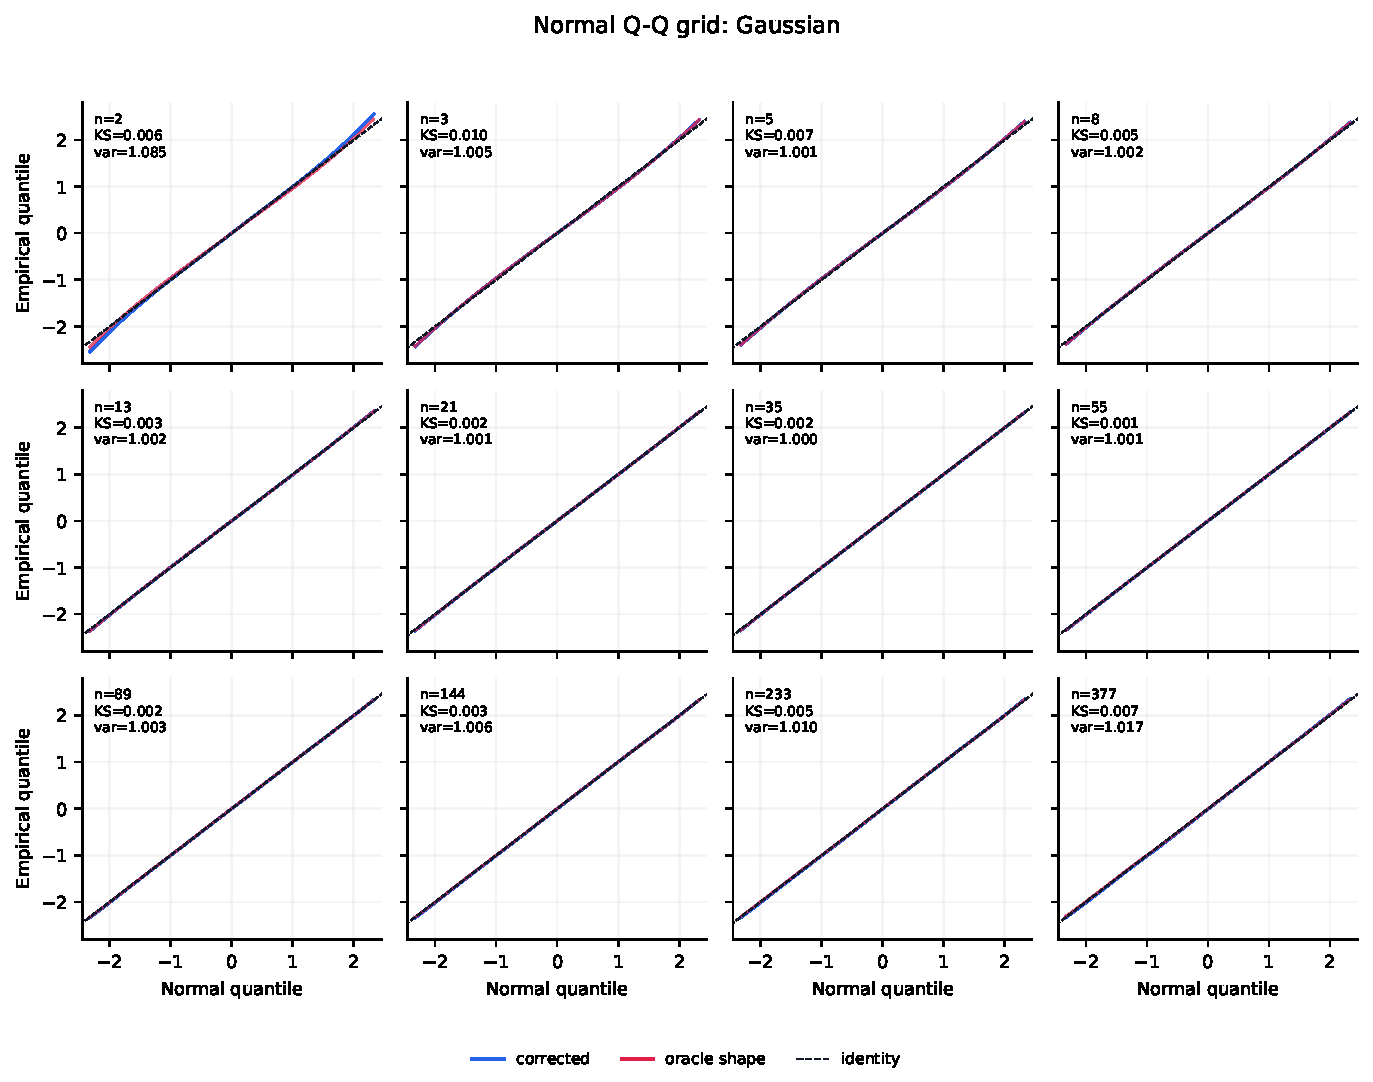
\includegraphics[height=0.385\textheight,keepaspectratio]{qq_grid_gaussian.pdf}
\par\vspace{-1mm}{\small (a) Gaussian innovations.}\par\vspace{1mm}
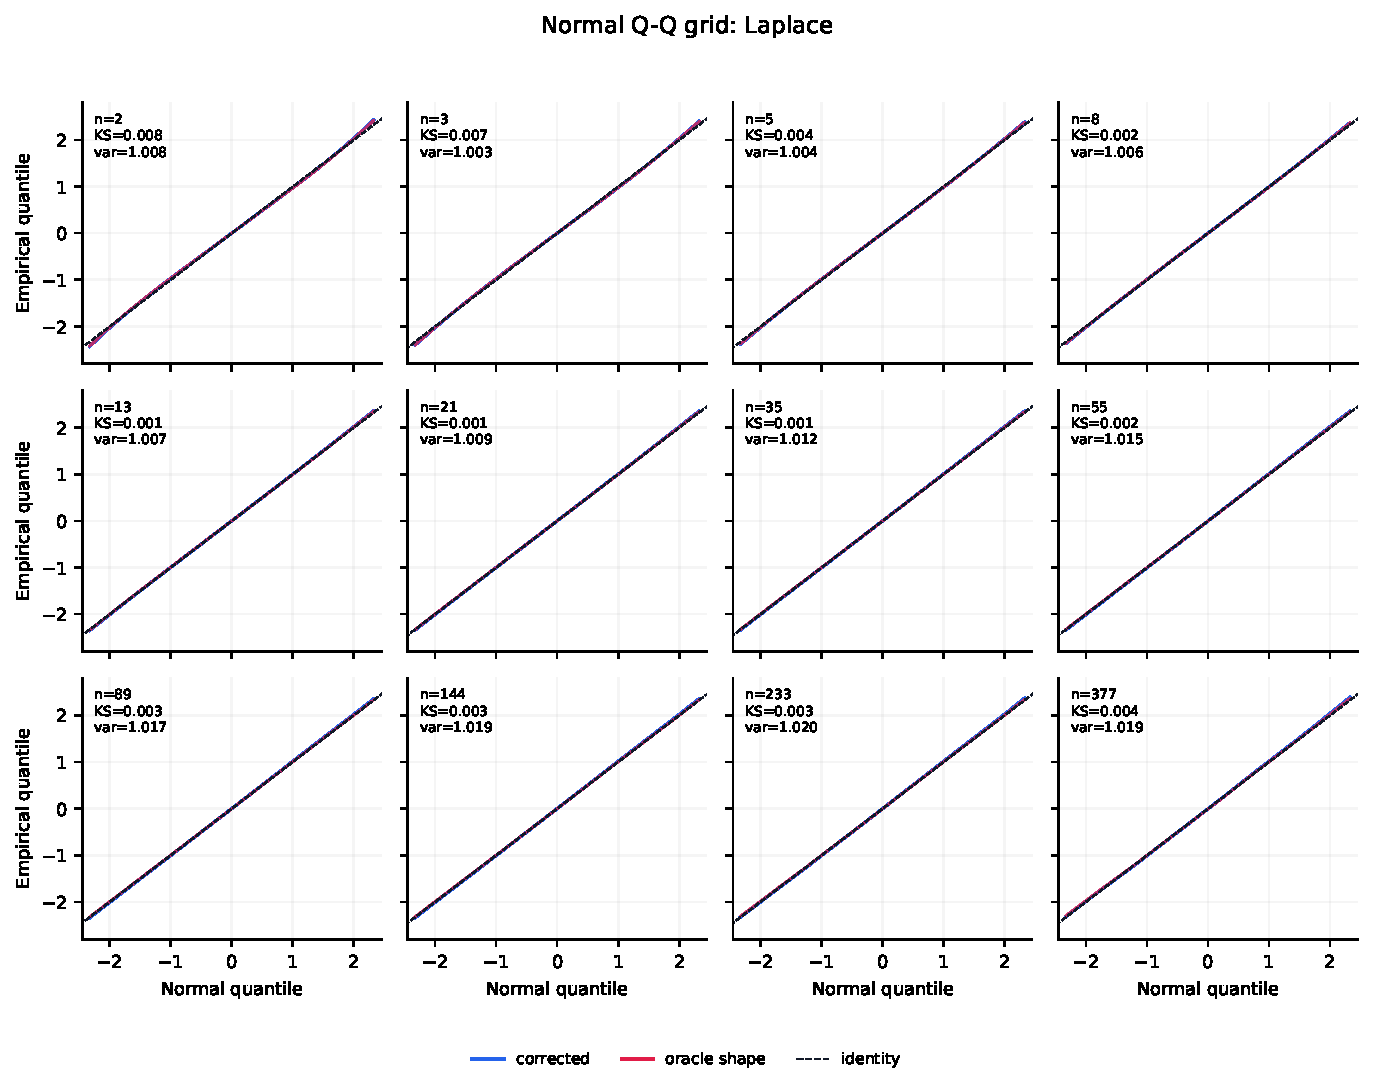
\includegraphics[height=0.385\textheight,keepaspectratio]{qq_grid_laplace.pdf}
\par\vspace{-1mm}{\small (b) Laplace innovations.}
\caption{Normal Q-Q grids for Gaussian and Laplace innovations.}
\end{figure}

\begin{figure}[p]
\centering
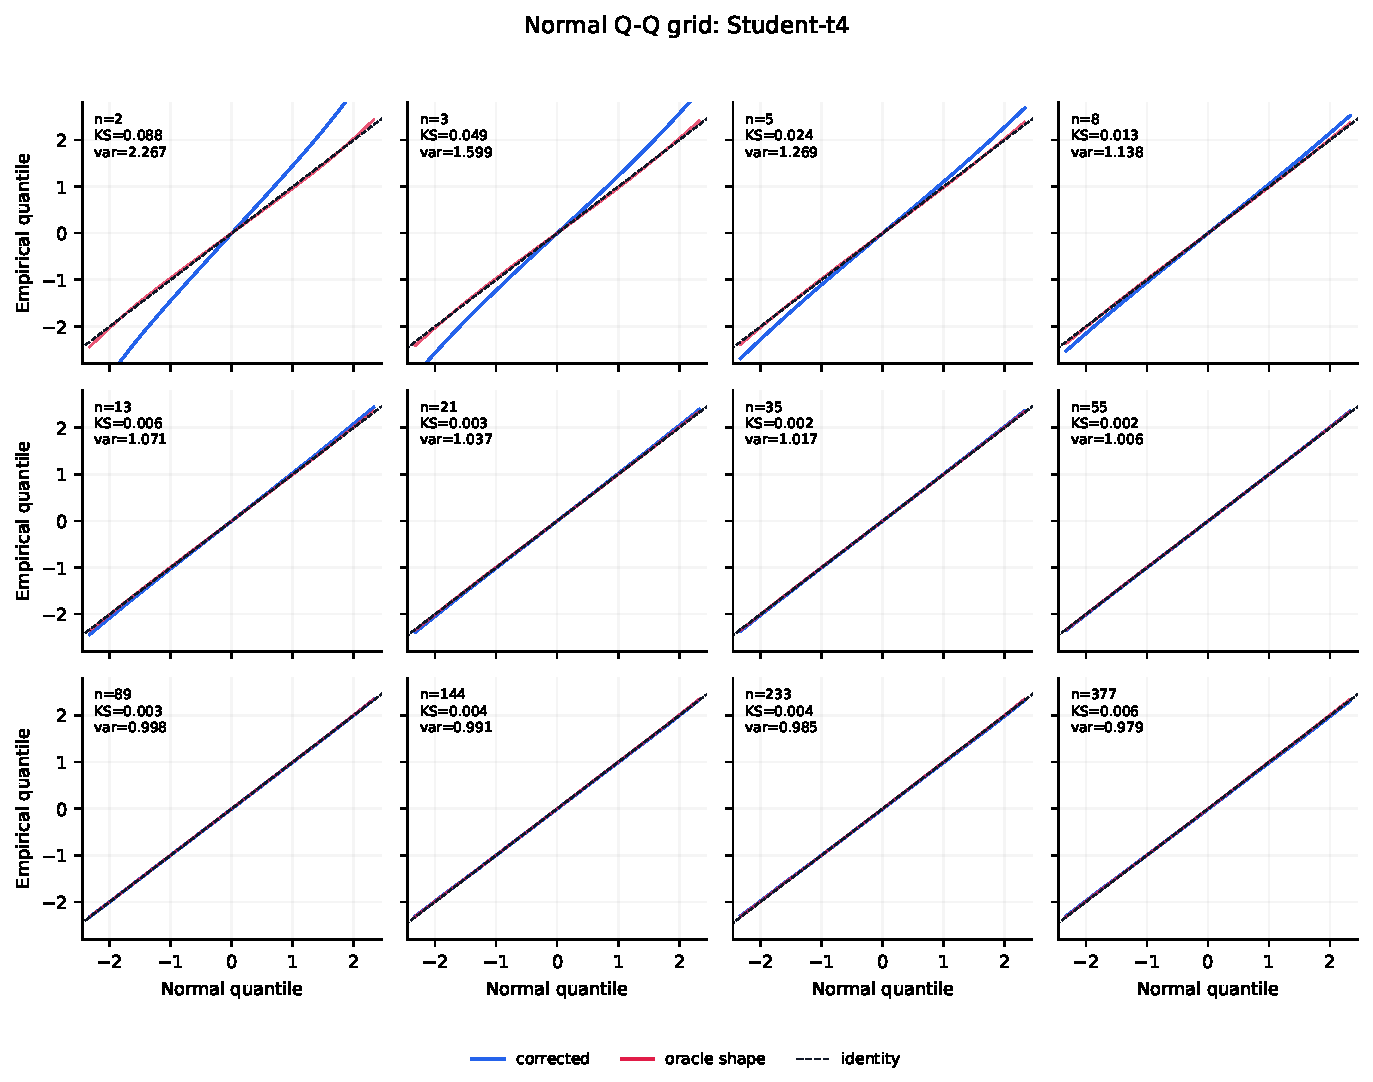
\includegraphics[height=0.385\textheight,keepaspectratio]{qq_grid_student_t4.pdf}
\par\vspace{-1mm}{\small (a) Student \(t_4\) innovations.}\par\vspace{1mm}
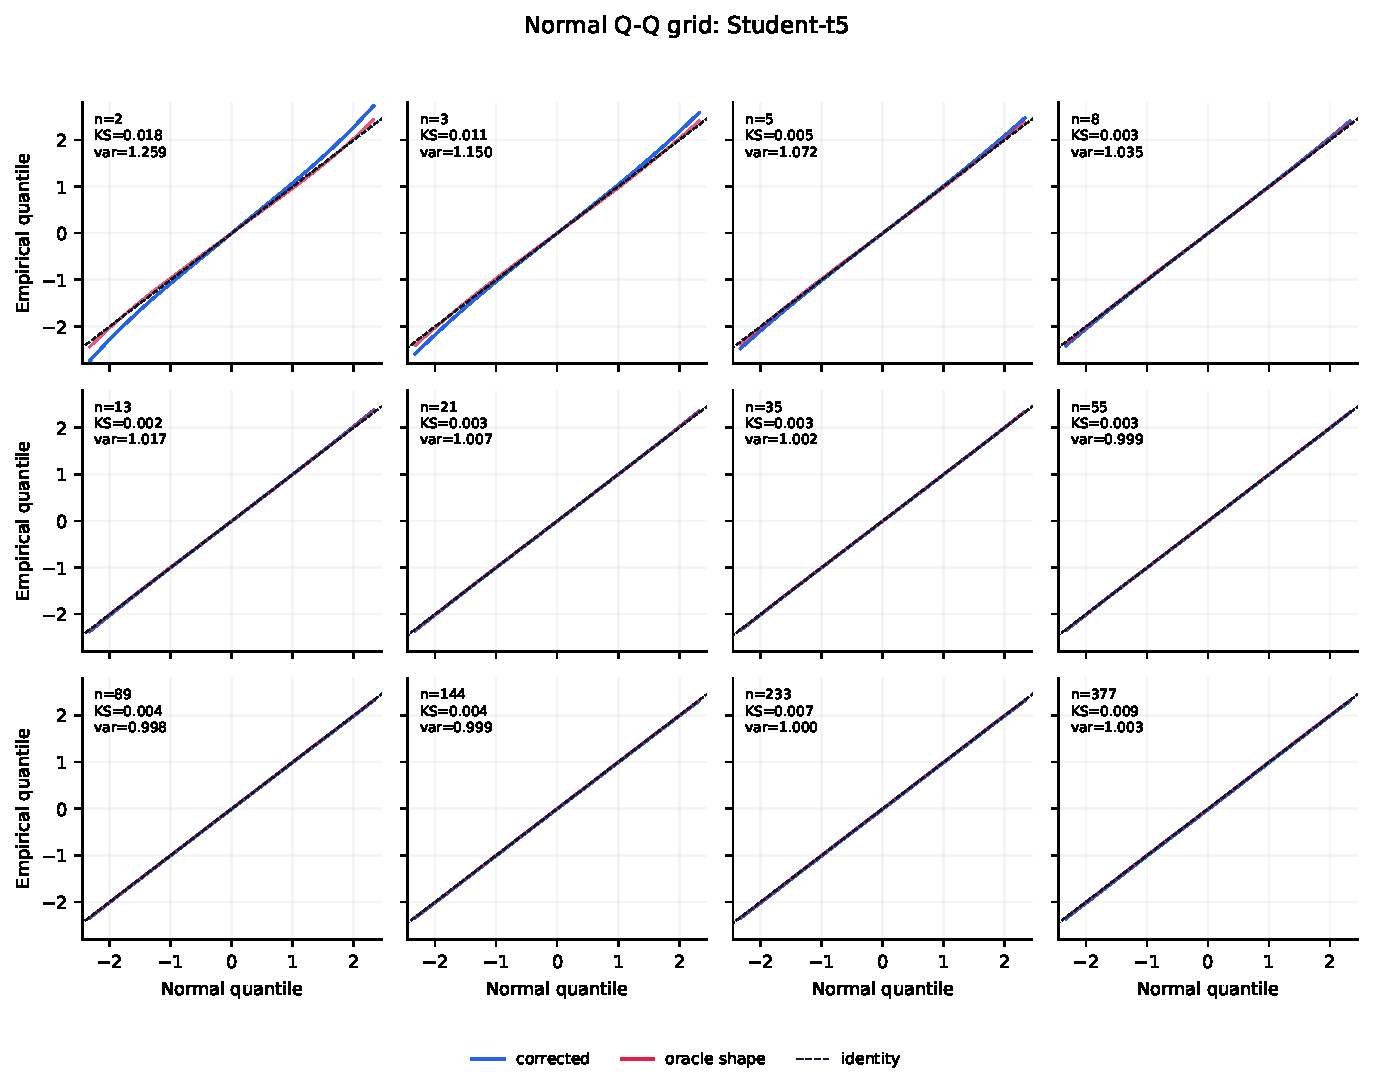
\includegraphics[height=0.385\textheight,keepaspectratio]{qq_grid_student_t5.pdf}
\par\vspace{-1mm}{\small (b) Student \(t_5\) innovations.}
\caption{Normal Q-Q grids for Student \(t_4\) and \(t_5\) innovations.}
\end{figure}

\begin{figure}[p]
\centering
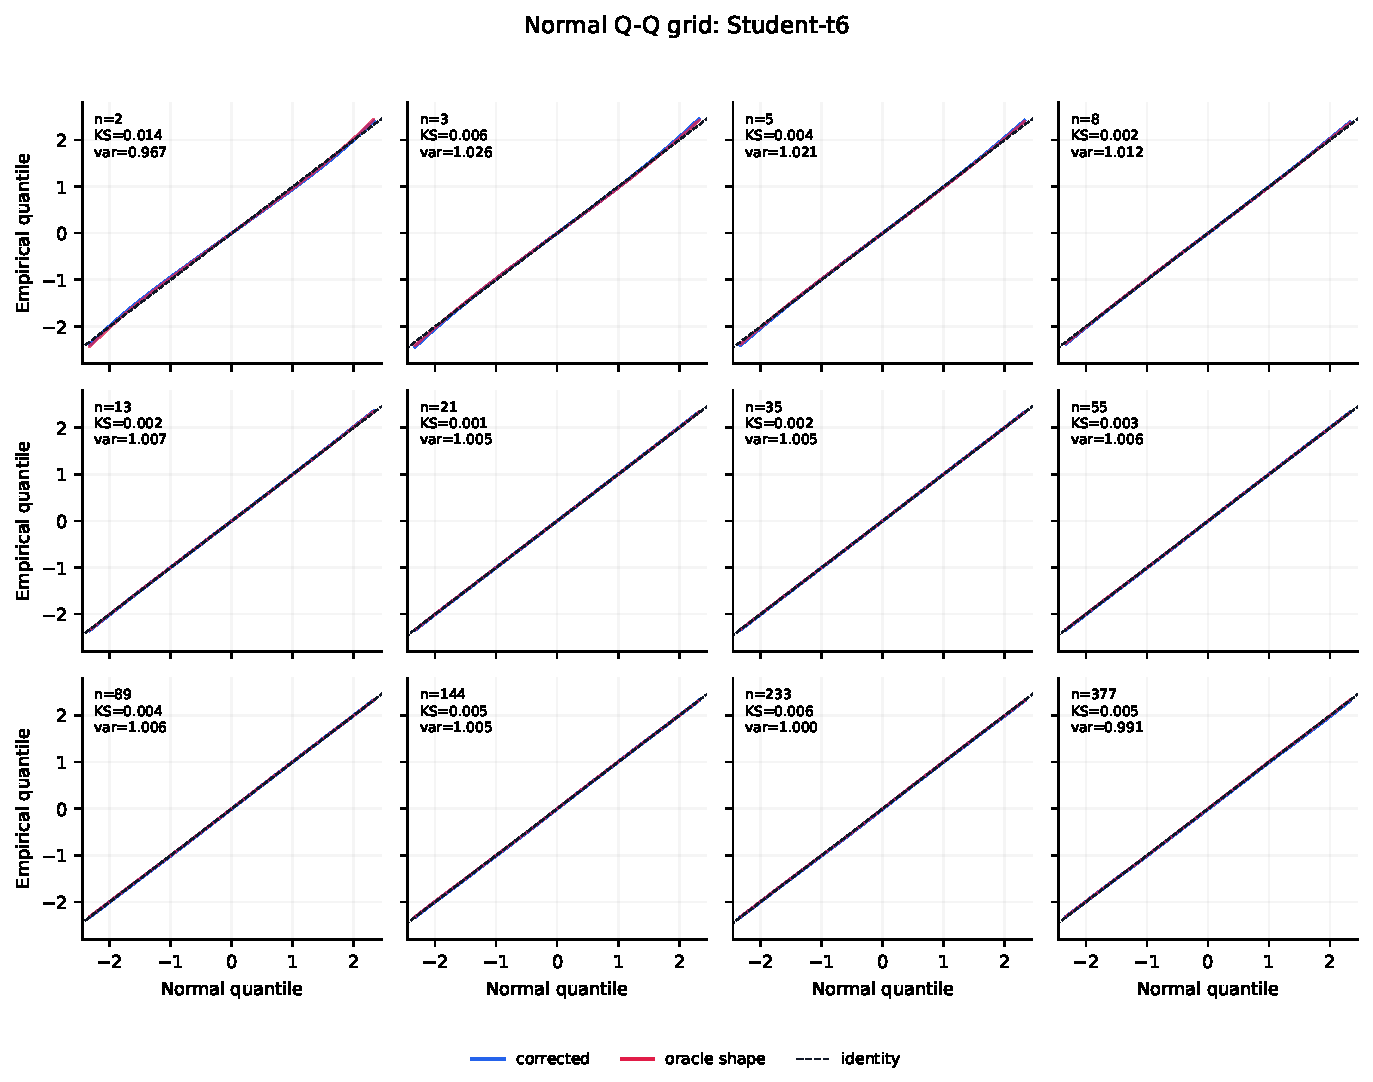
\includegraphics[height=0.385\textheight,keepaspectratio]{qq_grid_student_t6.pdf}
\par\vspace{-1mm}{\small (a) Student \(t_6\) innovations.}\par\vspace{1mm}
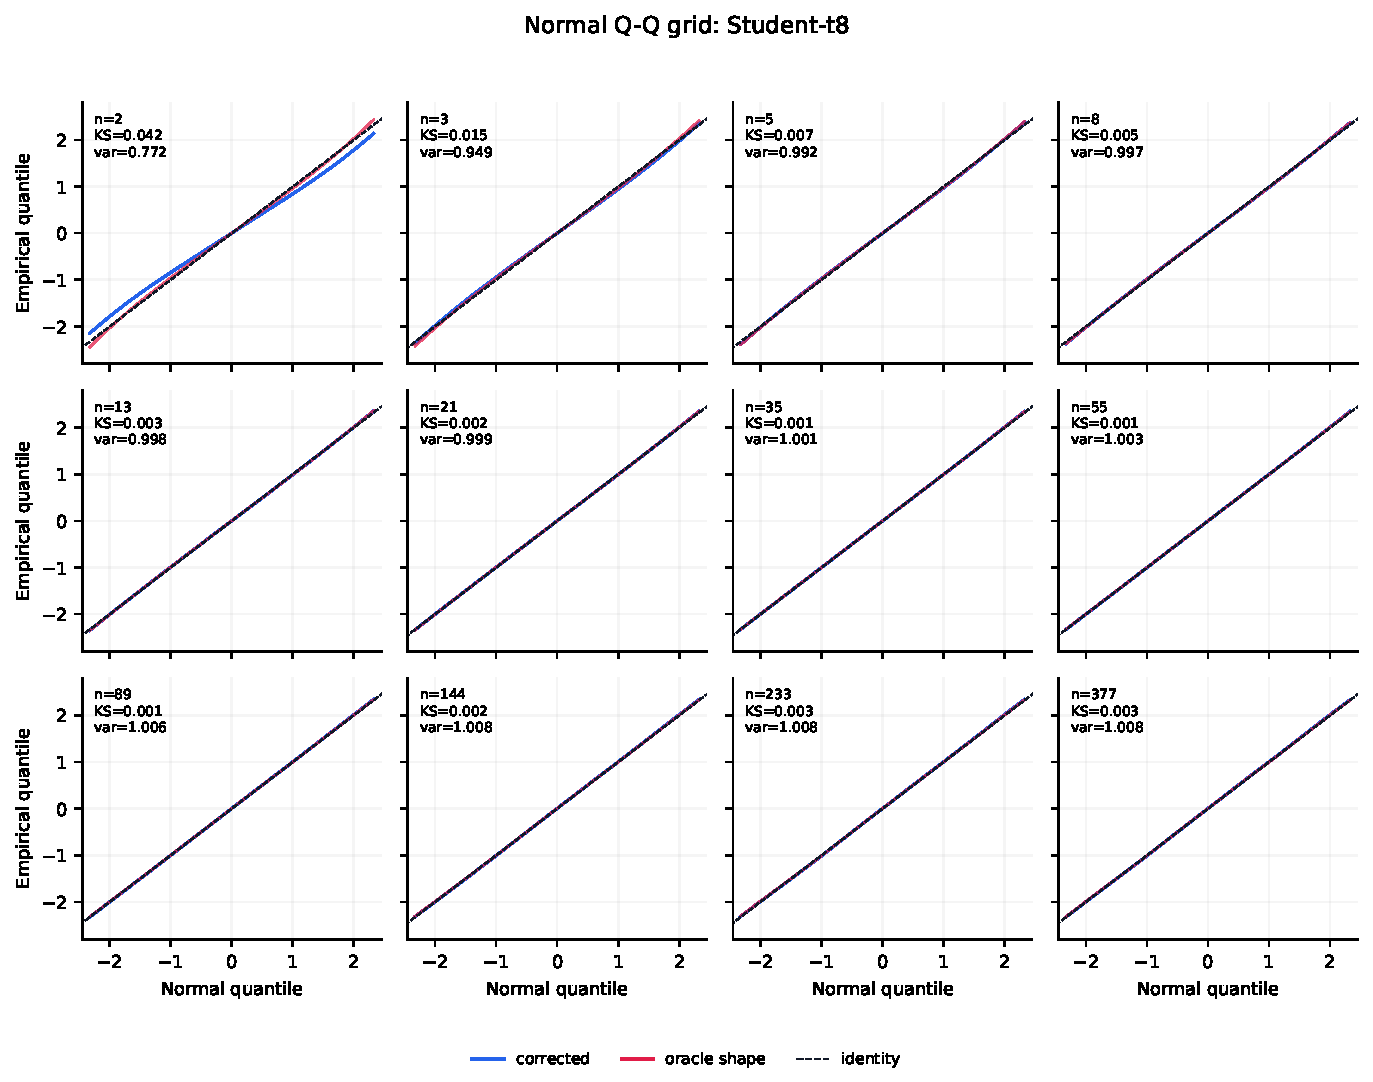
\includegraphics[height=0.385\textheight,keepaspectratio]{qq_grid_student_t8.pdf}
\par\vspace{-1mm}{\small (b) Student \(t_8\) innovations.}
\caption{Normal Q-Q grids for Student \(t_6\) and \(t_8\) innovations.}
\end{figure}

\clearpage
\section{Reproducibility and provenance}
\label{app:reproducibility}

On Windows, run the complete audit from the repository root with:
\begin{verbatim}
py -m pip install -r supplement\normality_audit\requirements.txt
py supplement\normality_audit\run_normality_audit.py
\end{verbatim}
On Linux or macOS, use:
\begin{verbatim}
python3 -m pip install -r supplement/normality_audit/requirements.txt
python3 supplement/normality_audit/run_normality_audit.py
\end{verbatim}
The archived reproducibility package contains summary metrics, quantile and
empirical-CDF grids, histogram counts, block summaries, representative draws,
the simulation configuration, machine-readable quality checks, tables,
figures, and source files.  All figures can be regenerated from the archived
aggregate outputs without rerunning the simulation:
\begin{verbatim}
py supplement\normality_audit\run_normality_audit.py --plots-only
\end{verbatim}
On Linux or macOS, replace \texttt{py} with \texttt{python3} and use forward
slashes in the same command.
\medskip
\noindent
The author formulated the research question, mathematical framework, and
interpretation, and takes responsibility for the claims made in this report.
AI tools assisted with computational design, code drafting, debugging,
visualization, and editorial preparation.  Numerical results were produced by
the archived code and preserved outputs; they are not Lean-verified theorems.

\end{document}
